\subsection{Impulsfahrplan}
\begin{figure}[h]
	\centering
	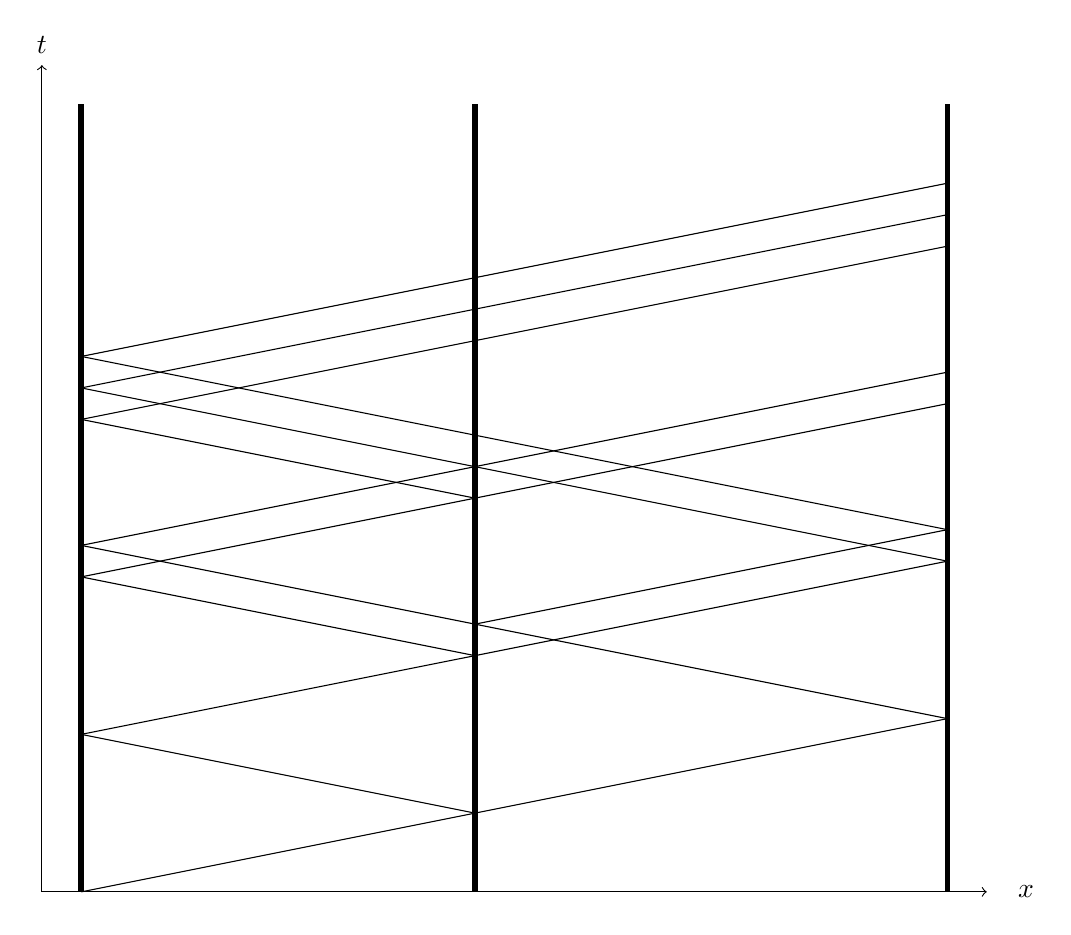
\begin{tikzpicture}
	\draw[line width=2pt] (0,0) -- (0,10);
	\draw[line width=2pt] (11,0) -- (11,10);
	\draw[line width=2pt] (5,0) -- (5,10);
	\draw[->] (-0.5,0) -- node [yshift = 5.5cm]{$t$} (-0.5,10.5);
	\draw[->] (-0.5,0) -- node [xshift = 6.5cm]{$x$} (11.5,0);
	% Linie1
	\draw (0,0) -- (11,1/5*11);
	\draw (11,1/5*11) -- (0,1/5*11*2);
	\draw (0,1/5*11*2) -- (11,1/5*11*3);

	% Linie2
	\draw (5,1) -- (0,2);
	\draw (0,2) -- (11,1/5*11+2);
	\draw (11,1/5*11+2) -- (0,1/5*11*2+2);
	\draw (0,1/5*11*2+2) -- (11,1/5*11*3+2);
	
	%Linie3
	\draw (5,3) -- (0,4);
	\draw (0,4) -- (11, 1/5*11+4);
%	\draw (11, 1/5*11+4) -- (0,1/5*11*2+4);
	
	%Linie4
	\draw (5,5) -- (0,6);
	\draw (0,6) -- (11,1/5*11+6);
	
	\draw (5,1/5*11*2-1) -- (11,1/5*11*2-1+1/5*6);
	\draw (11,1/5*11*2-1+1/5*6) -- (0,1/5*11*2-1+1/5*6+1/5*11);
	\draw (0,1/5*11*2-1+1/5*6+1/5*11) -- (11,1/5*11*2-1+1/5*6+1/5*11*2);
\end{tikzpicture} \\
	\caption[Impulsfahrplan]{Impulsfahrplan zur Veranschaulichung der Mehrfachreflexion}
	\label{fig:Impulsfahrplan}
\end{figure}
\subsection{Bestimmung der Reflexionskonstanten}
\begin{figure}[h]
	\centering
	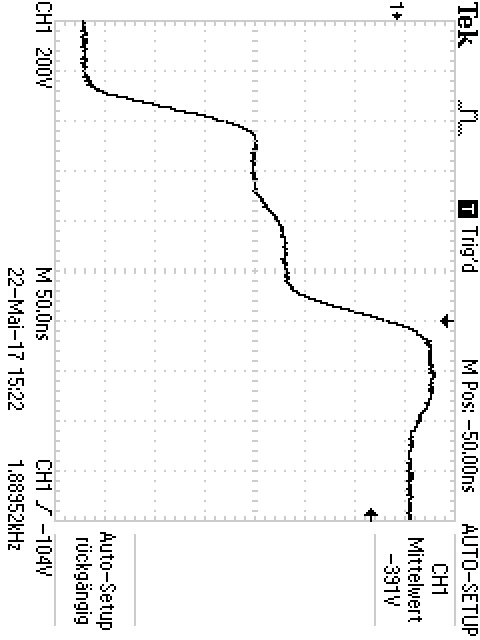
\includegraphics[width=0.5\textwidth]{Oszilloskop/Mehrfachreflexion/F0054TEK.JPG}
	\caption[Mehrfachreflexion]{Bild am Oszilloskop bei der Mehrfachreflexion}
	\label{fig:Mehrfachreflexion}
\end{figure}
LGS
\begin{align}
	\Delta U_1 &= \Gamma_{12}U_0 \\
	\Delta U_2 &= \Gamma_A\Gamma_{12}^2U_0 + (1-\Gamma_{21})\Gamma_E(1-\Gamma_{12})U_0 \\
	\Delta U_3 &= \Gamma_{12}\Gamma_A\Gamma_E(1-\Gamma_{21})(1-\Gamma_{12})U_0 + \Gamma_A^2\Gamma_{12}^3U_0 \\
%	&+ (1-\Gamma_{21})\Gamma_E(1-\Gamma_{12})\Gamma_A\Gamma_{12}U_0 + (1-\Gamma_{21})\Gamma_E^2\Gamma_{21}(1-\Gamma_{12})U_0
\end{align}
Annahme: perfekte Transmission an A, d.h. $\Gamma_A=0$ (rote Linien)
\begin{align}
	\Delta U_1 &= \Gamma_{12}U_0 \\
	\Delta U_2 &= (1-\Gamma_{21})\Gamma_E(1-\Gamma_{12})U_0 \\
	\Delta U_3 &= (1-\Gamma_{21})\Gamma_E^2\Gamma_{21}(1-\Gamma_{12})U_0
\end{align}
Lösung
\begin{align}
	\Gamma_{12} &= \frac{\Delta U_1}{U_0} \\
	\Gamma_{21} &= \frac{1}{1+\frac{\Delta U_2^2}{\Delta U_3(U_0-\Delta U_1)}} \quad, \Gamma_E \not= 0\text{ (unphysikalisch)}, \Delta U_1 \not= U_0\text{ (unphysikalisch)} \\
	\Gamma_E &= \frac{\Delta U_3}{\Delta U_2} + \frac{\Delta U_2}{U_0-\Delta U_1}
\end{align}
Theorie
\begin{align}
	\Gamma_E &= 1 \\
	\Gamma_A &= ?? \\
	\Gamma_{12} &= 0.1\overline{8} \\
	\Gamma_{21} &= -0.1\overline{8}
\end{align}
\todo{Bei mir kompiliert Latex nicht richtig, wenn ich dieses Bild einbinde...}
%\begin{figure}[h]
%	\centering
%	\input{Mehrfachreflexion/build/Plot.pdf}
%	\caption{text}
%	\label{fig:U}
%\end{figure}
\begin{align}
	U_0 &= \SI{-1.81994+-0.00002}{\kilo\volt}
 \\
	U_1 &= \SI{-1.1}{\kilo\volt}
 \\
	U_2 &= \SI{119.04+-0.03}{\volt}
 \\
	U_3 &= \SI{-0.4}{\kilo\volt}
 \\
\end{align}
\subsection{Bestimmung der Kabellängen}
$T$ ist die Zeit zwischen zwei Signalen (Abstand zwischen den Anfängen der Plateaus):
\begin{align}
	T_1 &= \SI{0.108}{\micro\second}
 \\
	T_2 &= \SI{0.093}{\micro\second}
 \\
	T_3 &= \SI{0.114}{\micro\second}
 \quad.
\end{align}
Es gelten die Beziehungen (siehe Impulsfahrplan \ref{fig:Impulsfahrplan})
\begin{align}
	T_1 &= \frac{2L_1}{v} \\
	T_2 &= \frac{2L_1 + 2L_2}{v}-T_1 = \frac{2L_2}{v} \\
	T_3 &= \frac{2L_1+4L_2}{v}-T_2 = \frac{2L_2}{v} \quad.
\end{align}
Nach den Längen aufgelöst ergibt sich so
\begin{align}
	L_1 &= \SI{10.8}{\meter}
 \\
	L_2 &= \SI{10.3+-0.7}{\meter}
 \quad, 
\end{align}
wobei $L_2$ einmal mit $T_2$ und einmal mit $T_3$ ausgerechnet wurde und hier der Mittelwert steht.